\subsection{Hjørner}\label{subsec:corner}
At detektere hjørner er en udbredt teknik indenfor feature detektion, da hjørner ofte forekommer i forskellige menneskeskabte scener og fordelagtigt kan bruges i disse sammenhæng. Et hjørne kan defineres som et område i og omkring et punkt, der har to dominerede kantretninger (kanter bliver nærmere bestemt i sektion 3.1.2). Hjørner er interessepunker, hvis de er distinktive og repeterbare. Førstnævnte kan vises, ved at betragte hvordan et hjørne identificeres:
\begin{figure}[H]
    \centering
    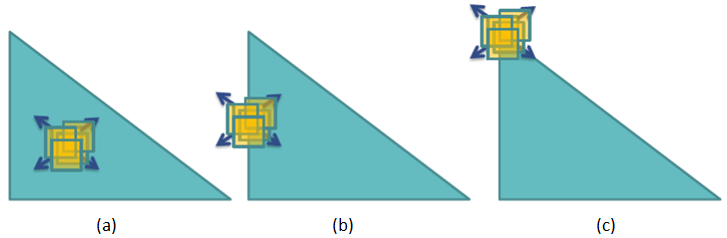
\includegraphics[width=0.55\textwidth]{fig/6.png}
    \vspace{-1em}   
    \begin{center}    
    \caption{\textcolor{gray}{\footnotesize \textit{
     Tre udvalgte vinduer, med interessepunkter i centrum af samme motiv. \textbf{(a)} Punktet er lokaliseret i en teksturløs region, d.v.s. ingen teksturskift. \textbf{(b)} Punktet er lokaliseret på en kant. \textbf{(c)} Punktet er lokaliseret på et hjørne }}}
    \label{fig:2}
     \end{center}
    \vspace{-2.7em}  
  \end{figure}  
\noindent
I figur \ref{fig:2} ses tre udvalgte punkter med et dataindsamlingsvindue placeret over. For at lokalisere et hjørne, forskydes dataindsamlingsvinduet med en enkelt pixelværdi, i otte retninger (syd, sydøst, øst, osv), og billedintensiteten sammenlignes med originalvinduet, der ikke er forskudt - et hjørne identificeres ved, at et skift i alle retninger, danner otte vinduer, hvis intensitet er forskelligt fra hver andre.???
	
. Forskydes  \textbf{(a)}, uanset retning, vil alle forskudte vinduer være identiske, da punktet og regionen omkring er homogent. Punktet er derfor ikke interessant. Forskydes \textbf{(b)} i x-aksen vil der opstå en region der ikke identisk med den originale, men en forskydning i y-aksen vil resultere i en region identiske med den originale, og punktet er derfor ikke interessant. Punktet placeret på et hjørne \textbf{(c)} er interessant en forskydninger uanset retning, vil resultere i en region, der ikke er identisk med den originale. Hjørnet kan derfor bruges som et interessepunkt. Denne intuitive definition kan kvantificeres til en matematisk definition, der estimere auto-korrelationen imellem de forskudte billeder, hvilket angiver intensitetsskiftene imellem billederne og derved angivers hvor der opstår et hjørne.


Hvis det antages, at der forekommer en begrænset mængde hjørner i et billede, kan et hjørne bruges som interessepunkt, da lever op til kravet om repeterbarhed. <Om det er distinktivt, kan diskuteres>.